\documentclass{standalone}
\usepackage{standalone}

\begin{document}
\chapter{Data Collection}

For any system to train with a dataset we have to collect data and organize them. So, data collection is one of the most important parts of research works. Therefore data collection is also important in speech recognition. There are plenty of data for English ASR and English corpses are available. But in Bangla, there are not plenty of data and corpses are not widely available.
So, it is challenging for building an ASR for Bangla language. A good corpus naming Speech Corpora of 125 hours segmented data set from 697 speakers are developed by Linguistic data consortium for Indian Languages(LDC-IL) \cite{shrishrimal2012indian}. But unfortunately, this is only available for LDC-IL authorized members. "SRUTI Bengali Continous ASR Speech corpus" is another valuable corpus for Bangla speech recognition. This is consisting of 21.64 hours \cite{das2011bengali}. That is available but in several linguistic contexts of Bangladeshi Bangla phonetically and contextually different from Indian,, Kolkata based Bangla. So we need a corpus and that's why we have collected an isolated word corpus.

Then the research work of "Pipilika" has come. We have got some isolate speech data from the previous work. We have got words from 81 speakers. The data set is not big enough. So, working from the beginning is necessary for Bangla ASR. For this, we have to build a standard system for making the model more efficient. We are very much grateful to our department and "Pipilika" for providing the fund and technology for building standard system. Our process of data collection is given below:

\section{Word Selection for corpus}
First of all, we want to develop a standard system for the ASR of Pipilika. From previous work, we have got 1000 unique words with 81 speakers. Here we have collected another 35 unique words and our number of speakers is 91. We follow the instructions of our supervisor for collecting the data.
Our collected dataset consists of some data of most frequent words provided by Pipilika office. Some online articles and newspapers provided keywords which are mostly search in our country. We include mostly the celebrity names, sportsman and tourists spots in our corpus. Then we mapped the words with an individual unique number. Further, we collected the audio data of the unique words and build a corpus.

\begin{figure}[h]
 \centering
 \centerline{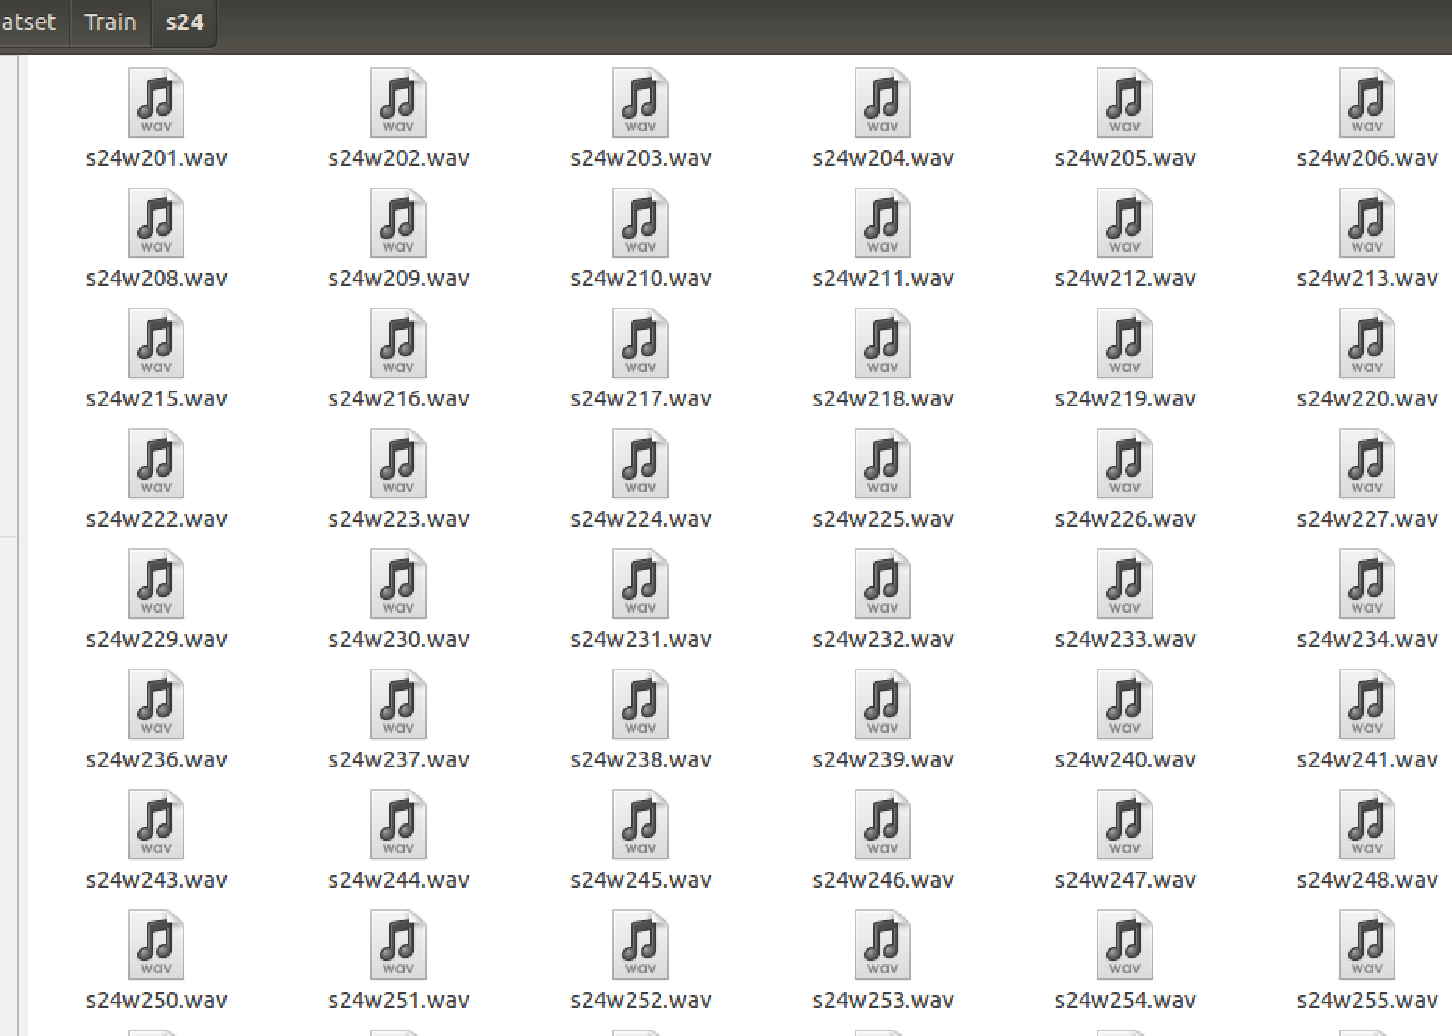
\includegraphics[width=13cm, height=6.5cm]{img/WavFile.pdf}}
 \caption{Speech Corpus}
\label{fig:speech-corpus}
\end{figure}


\section{Speakers Detail}
  In our collected dataset, we have got 62 male and 29 female speakers data. So, the ratio of the female and male speakers is 32\% : 69\%. So far we have got the knowledge that if we are able to collect almost 40\% and 60\% data of female and male speakers then we should get a better accuracy \cite{hinton2012deep}.
  In our corpus, we have tried to emphasize both the male and female speakers. We have collected the data from various ages as people around the university area between 19-25 years.

\section{Recording}
 We have used an open source software called Praat for recording. 
The recording speeches are 24000Hz. Each speaker was said to record the words as their general vocal as they pronounced that in their daily life. We prefer at least 100 words for each speaker which consist of 3 same words. In our thesis, we have collected 250 voices from one speaker for a unique 250 words. Thus for 1000 words, there were 4 speakers and for rest of the 35 words, there was one speaker. Thus we have collected 2070 voices from all 10 different female speakers.

\section{Extract Word From Sentences}
We recorded 3 utterances as a sentence in a wav file then divide it into words. We split sentences based
on silence between words. We use SOX tool for splitting the sentence. Be default Kaldi internally handle this process.

\end{document}